\documentclass{beamer}

% don't display the beamer navbar
\usenavigationsymbolstemplate{}

\usepackage[latin1]{inputenc}
\usepackage[T1]{fontenc}
\usepackage{ae}

%Candidates: Antibes, Bergen, Berkeley, Berlin, Boadilla, Copenhagen, Darmstadt, Dresden,
%            Frankfurt, Goettingen, Hannover, Ilmenau, JuanLesPins, Madrid, Malmoe, Marburg,
%            Montpellier, PaloAlto, Pittsburgh, Rochester, Singapore, Szeged, Warsaw
%
% see: http://mike.polycat.net/gallery/beamer-themes for an overview
\usetheme{Darmstadt}

\usepackage{xmpmulti}
%\usepackage{multimedia}

\title[pNLP]{practical Natural Language Processing}
\subtitle{\medskip krdwrd {\tiny \cite{asn-spatz.de, krdwrd.org}}
}
\author[maria, kilian and egon]{Maria Cieschinger, Kilian Klimek and Egon Stemle} % {\footnotesize \texttt{<egon.stemle@uos.de>}}}
\date{May 22, 2008}
\institute{
Institute of Cognitive Science \\
University of Osnabr�ck
}

%
%DOCUMENT begins here
%
\begin{document}

\begin{frame} % [shrink=10]
	\titlepage
	
%	\begin{center}
%		{\tiny last update on \today}
%	\end{center}
\end{frame}


%%%%%%
%
%CONTENT comes here
%

%
%egon

%\part{Motivation}
	%\frame{\partpage}
	%\begin{frame}
	%	\frametitle{Outline}
	%	\tableofcontents
	%\end{frame}
	
	%\section[introduction]{Introduction}
\section*{}
\subsection*{}

%\begin{frame}[shrink=1]

\begin{frame}
	\frametitle{History and Motivation}
		
		CLEANEVAL-1 was a shared task and competition on the topic of cleaning arbitrary web pages
		
	\begin{block}{}	
		\begin{itemize}
			\item The goal was to prepare web data for use as a corpus, for linguistic and language technology research and development
			\pause
			\item[$\rightarrow$] We don't question \emph{this goal}.
		\end{itemize}
	\end{block}
\end{frame}

\begin{frame}[allowframebreaks]
	\frametitle{So far\ldots}
\begin{quote}
The World Wide Web offers a unique possibility to gather large amounts of authentic and
up-to-date language data from a wide variety of genres, and to build corpora containing
billions of words of text with relatively little effort. {\tiny \cite{FIASCO2007}}
\end{quote}

\framebreak

The large amount of data calls for ML techniques.
\begin{enumerate}
	\item Acquire/Prepare Training Data
	\item Pre-Processing of Data
	\item Learn/Classify
\end{enumerate}

\framebreak
\ldots but
	\begin{center}
		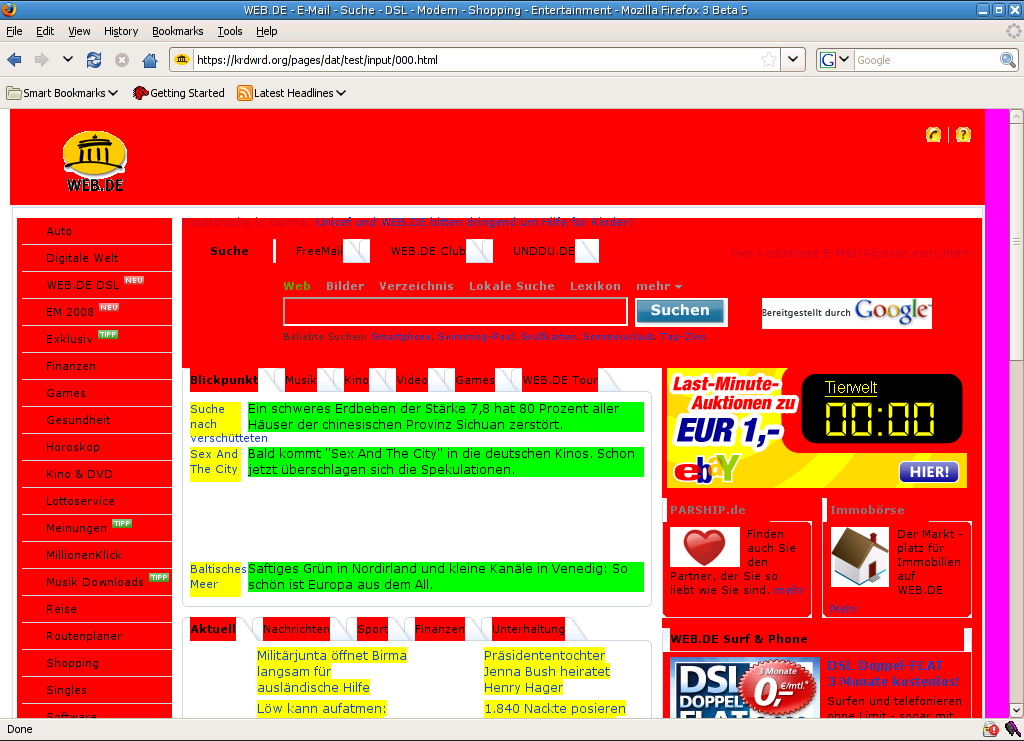
\includegraphics[height=0.7\textheight]{20080522_pics/shot1.png} %\\ {\tiny copied from \cite[Vorlesung 01, p.35]{emma.informatik.unibw-muenchen.de}}
	\end{center}

\framebreak

	\begin{center}
		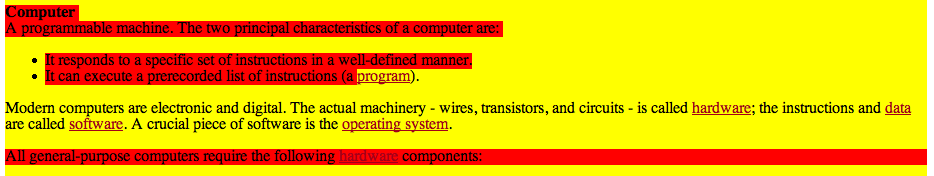
\includegraphics[width=\textwidth]{20080522_pics/bad.png} %\\ {\tiny copied from \cite[Vorlesung 01, p.35]{emma.informatik.unibw-muenchen.de}}
	\end{center}
\end{frame}


\begin{frame}
	\frametitle{A Solution.}
	\begin{center}
		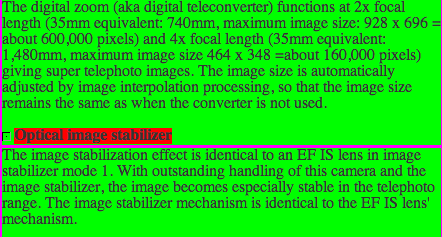
\includegraphics[width=\textwidth]{20080522_pics/good.png} %\\ {\tiny copied from \cite[Vorlesung 01, p.35]{emma.informatik.unibw-muenchen.de}}
	\end{center}
\end{frame}

\begin{frame}
	\frametitle{A Solution?}
	\begin{center}
		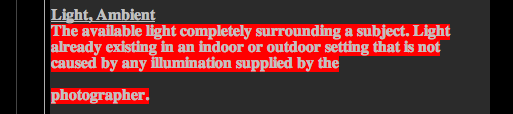
\includegraphics[width=\textwidth]{20080522_pics/evil.png} %\\ {\tiny copied from \cite[Vorlesung 01, p.35]{emma.informatik.unibw-muenchen.de}}
	\end{center}
\end{frame}

\begin{frame}
	\frametitle{Next Steps and Goals}

	\begin{itemize}
		\item Improve usability and functionality of Firefox Add-On
		\item Develop guidelines (aka. rewrite, disambiguate, enhance, etc. current ones)
		\item Tag pages (or rather have them tagged)
		\item[$\rightarrow$] Stay tuned on krdwrd.org {\tiny \cite{krdwrd.org}}.
	\end{itemize}
\end{frame}


%\part{Infrastructure}
%	\frame{\partpage}
%	\begin{frame}
%		\frametitle{Outline}
%		\tableofcontents
%	\end{frame}
%
%	\input{01_content}

%\part{}
%	\frame{\partpage}
%	
%	\begin{frame}
%		\frametitle{Outline}
%		\tableofcontents
%	\end{frame}
%
%
%	\input{02_content}

%
%
%%%

%\begin{frame}{frametitle}{framesubtitle}
%\end{frame}
%\input{99_test}

%%%
% REFERENCES
%
%\part{References}
	%\frame{\partpage}

	%\section[references]{References}
	\begin{frame}[allowframebreaks]
		\frametitle{References}
	
		\setbeamertemplate{bibliography item}[text]
		\footnotesize
		\bibliographystyle{alphaurl}
		\bibliography{2008.pNLP}
		% \nocite{*}
	\end{frame}
%
%%%

\end{document}
